\documentclass[11pt,twoside]{article}
\usepackage[english]{babel}
\usepackage{times,subeqnarray}
\usepackage{url}
%\usepackage{lineno}
% following is for pdflatex vs. old(dvi) latex
\newif\myifpdf
\ifx\pdfoutput\undefined
%  \pdffalse           % we are not running PDFLaTeX
   \usepackage[dvips]{graphicx}
\else
   \pdfoutput=1        % we are running PDFLaTeX
%  \pdftrue
   \usepackage[pdftex]{graphicx}
\fi
\usepackage{apatitlepages}
% if you want to be more fully apa-style for submission, then use this
%\usepackage{setspace,psypub,ulem}
\usepackage{setspace} % must come before psypub
%\usepackage{psypub}
\usepackage{psydraft}
%\usepackage{one-in-margins}  % use instead of psydraft for one-in-margs
\usepackage{apa}       % apa must come last
% using latex2e as standard, use the following for latex209
% \documentstyle [times,11pt,twoside,subeqnarray,psydraft,apa,epsf]{article}
%\input netsym

% tell pdflatex to prefer .pdf files over .png files!!
\myifpdf
  \DeclareGraphicsExtensions{.pdf,.eps,.png,.jpg,.mps,.tif}
\fi

% use 0 for psypub format 
\parskip 2pt
% for double-spacing, determines spacing 
% \doublespacing
% \setstretch{1.5}
\columnsep .25in   % 3/8 in column separation

\def\myheading{ Deep Predictive Learning }

% no twoside for pure apa style, use \markright with heading only
\pagestyle{myheadings}
\markboth{\hspace{.5in} \myheading \hfill}{\hfill O'Reilly, Russin, \& Rohrlich \hspace{.5in}}

%\bibliographystyle{pnas-new}

\def\mytitle{ Deep Predictive Learning in Neocortex and Pulvinar}

\def\myauthor{Randall C. O'Reilly, Jacob L. Russin, and John Rohrlich\\
  Department of Psychology, Computer Science, and Center for Neuroscience \\
  University of California Davis \\
  1544 Newton Ct\\
  Davis, CA 95618\\
  {\small oreilly@ucdavis.edu}\\}

% Please add here a significance statement to explain the relevance of your work
% \significancestatement{We present a significant advance in understanding how the human brain learns, based on the idea that canonical circuits between the neocortex and thalamus drive alternating phases of prediction and bottom-up outcomes, and the resulting prediction errors (as differences in activation states over time) can drive powerful learning.  Critically, we show for the first time that learning based solely on predicting raw visual inputs can generate higher-level abstract categorical representations of 3D objects, which previously has required explicit human-labeled training.  This captures the seemingly magic way in which human learning can create knowledge out of raw experience, without explicit teaching.}

% Please include corresponding author, author contribution and author declaration information
% \authorcontributions{RCO developed the model, performed the non-PredNet simulations, and drafted the paper. JLR performed the PredNet simulations and analysis, and edited the paper.  JR contributed to developing the model and edited the paper.}
% \authordeclaration{R. C. O'Reilly is Chief Scientist at eCortex, Inc., which may derive indirect benefit from the work presented here.}
% \correspondingauthor{\textsuperscript{1}To whom correspondence should be addressed. E-mail: oreilly@ucdavis.edu}

% Keywords are not mandatory, but authors are strongly encouraged to provide them. If provided, please include two to five keywords, separated by the pipe symbol, e.g:
% \keywords{Computational Modeling $|$ Predictive Learning $|$ Object Recognition $|$ Pulvinar $|$ Neocortex } 

\def\mynote{
We thank Dean Wyatte, Tom Hazy, Seth Herd, Kai Krueger, Tim Curran, David Sheinberg, Lew Harvey, Jessica Mollick, Will Chapman, Helene Devillez, and the rest of the CCN Lab for many helpful comments and suggestions.
Supported by: ONR grants ONR N00014-19-1-2684 / N00014-18-1-2116, N00014-14-1-0670 / N00014-16-1-2128, N00014-18-C-2067, N00014-13-1-0067, D00014-12-C-0638.  This work utilized the Janus supercomputer, which is supported by the National Science Foundation (award number CNS-0821794) and the University of Colorado Boulder. The Janus supercomputer is a joint effort of the University of Colorado Boulder, the University of Colorado Denver and the National Center for Atmospheric Research.
All data and materials will be available at \url{https://github.com/ccnlab/deep-obj-cat} upon publication.}

\def\myabstract{
How does the human brain learn new concepts from raw sensory experience, without explicit instruction?  We still do not have a widely-accepted answer to this central question.  Here, we propose a detailed biological mechanism for the widely-embraced idea that learning is based on the differences between predictions and actual outcomes (i.e., \emph{predictive error-driven learning}).  Specifically, numerous weak projections into the pulvinar nucleus of the thalamus generate top-down predictions, and sparse, strong \emph{driver} inputs from lower areas supply the actual outcome, originating in layer 5 intrinsic bursting (5IB) neurons. Thus, the outcome is only briefly activated, roughly every 100 msec (i.e., 10 Hz, \emph{alpha}), resulting in a \emph{temporal difference error signal}, which drives local synaptic changes throughout the neocortex, resulting in a biologically-plausible form of error backpropagation learning.  We implemented these mechanisms in a large-scale model of the visual system, and found that the simulated inferotemporal (IT) pathway learns to systematically categorize 3D objects according to invariant shape properties, based solely on predictive learning from raw visual inputs.  These categories match human judgments on the same stimuli, and are consistent with neural representations in IT cortex in primates.
}

\begin{document}
\bibliographystyle{apa}

% sloppy is the way to go!
% \sloppy
% \raggedbottom

\titlesepage{\mytitle}{\myauthor}{\mynote}{\myabstract}

\pagestyle{myheadings}

The fundamental epistemological conundrum of how knowledge emerges from raw experience has challenged philosophers and scientists for centuries.  There have been significant advances in understanding the detailed biochemical basis of learning in terms of synaptic plasticity between neurons \cite{LuscherMalenka12}, and many cognitive and computational models of learning.  However, there is still no widely-accepted answer to this puzzle, that is clearly supported by known biological mechanisms and also produces effective learning at computational and cognitive levels.  At these functional levels, the idea that we learn via an active \emph{predictive} process goes back to Helmholtz's \emph{recognition by synthesis} proposal \cite{Helmholtz13}, and has been widely embraced in a wide range of different frameworks \cite{Elman90,ElmanBatesKarmiloff-SmithEtAl96,Mumford92,DayanHintonNealEtAl95,RaoBallard99,KawatoHayakawaInui93,Friston05}.  

Here, we propose a detailed biological mechanism for a specific form of \emph{predictive error-driven learning} based on distinctive patterns of connectivity between the neocortex and the pulvinar nucleus of the thalamus \cite{ShermanGuillery06,UsreySherman18}.  Specifically, numerous weak projections into the thalamic relay cells (TRCs) in the pulvinar drive top-down predictions, and sparse, strong \emph{driver} inputs from lower areas encode the actual outcome, and learning is based on the difference.  Because these driver inputs originate in layer 5 intrinsic bursting (5IB) neurons, the outcome is only briefly activated, roughly every 100 msec (i.e., 10 Hz, \emph{alpha}).  Thus, the prediction error is a \emph{temporal difference} in activation states over the pulvinar, from an earlier prediction to a subsequent burst of outcome.  This temporal difference can drive local synaptic changes throughout the neocortex, supporting a biologically-plausible form of error backpropagation learning \cite{OReilly96,AckleyHintonSejnowski85,HintonMcClelland88,BengioMesnardFischerEtAl17,WhittingtonBogacz19,LillicrapSantoroMarrisEtAl20}. 

One primary objective of this paper is to describe this biologically-based mechanism for predictive error-driven learning in sufficient detail that it can be clearly evaluated relative to a wide range of existing anatomical and electrophysiological data.  We provide a number of specific empirical predictions that follow from this functional view of the thalamocortical circuit, which could potentially be tested by current neuroscientific methods.  Thus, a major contribution of this work is to provide a clear functional role for this distinctive thalamocortical circuitry that contrasts with existing ideas about what it might be doing, in testable ways.

A second major objective is to implement this predictive error-driven learning mechanism in a computational model that faithfully captures its essential biological features, while still being sufficiently simplified computationally that it can be used to simulate large-scale brain networks, to test whether the learning mechanism can drive the formation of cognitively-useful representations.  In particular, there is a critical question for any purely predictive-learning model: can it develop high-level, abstract ways of representing the raw sensory inputs, while learning from nothing but predicting these low-level visual inputs.  For example, most current models of visual object recognition that have been compared against neurophysiological data rely on large human-labeled image datasets to explicitly train abstract category information via error-backpropagation \cite{CadieuHongYaminsEtAl14,RajalinghamIssaBashivanEtAl18}.  Existing predictive-learning models based on error backpropagation \cite{LotterKreimanCox16} have not clearly demonstrated the development of abstract, categorical representations without additional human-labeled training.  Instead, previous work has shown that predictive learning can be a useful method for pretraining networks that are subsequently trained using human-generated labels.

Through large-scale simulations based on the known structure of the visual system, we found that our biologically based predictive learning mechanism developed high-level abstract representations that systematically categorize 3D objects according to invariant shape properties, based on raw visual inputs alone.  We found that these categories match human judgments on the same stimuli, and are consistent with neural representations in inferotemporal (IT) cortex in primates \cite{CadieuHongYaminsEtAl14}.  Furthermore, we show that comparison predictive DCNN models lacking these biological features \cite{LotterKreimanCox16} did not learn object categories that go beyond the visual input structure.  Thus, it is possible that incorporating certain biological properties of the brain can potentially provide a better understanding of human learning at multiple levels relative to existing DCNN models.  However, it is important to emphasize that our objectives in this work are \emph{not} to produce a better machine-learning (ML) algorithm per se, but rather to test the computational properties of our biologically-based, scientific theory for how the mammalian brain might learn.  Thus, we explicitly dissuade readers from the inevitable desire to evaluate the importance of our model based on differences in narrow, performance-based ML metrics: it should instead be evaluated on its ability to explain a wide range of data across multiple levels of analysis, just as every other scientific theory is evaluated.

The remainder of the paper is organized as follows.  First, we provide a concise overview of the biologically based predictive error-driven learning framework.  Next, we discuss the relevant biological data in detail, along with testable predictions that can differentiate this account of what this system does relative to existing ideas.  Then, we present the large-scale model of the visual system, which learns by predicting over brief visual movies of 3D objects rotating and translating over time and space.  We find that the model develops strongly categorical, shape-based representations in its upper IT layers, and these match those of human participants evaluating the same 3D objects.  Furthermore, we show that these categorical representations diverge significantly from the similarity structure present in the lower layers of the network.  Thus, we conclude that this form of predictive error-driven learning is capable of going beyond the surface structure of the raw sensory input, to develop higher-level abstract representations that otherwise have only been produced in neural models through explicit training via human-labeled image datasets.  To further explore this space, we evaluated two other prediction-error learning models using pure error-backpropagation, based on current deep-convolutional neural network (DCNN) principles, and found that they did not develop the same kind of high-level categories, and instead remained largely tied to the similarity structure of the raw visual inputs.  Thus, there may be some important features of the biologically-based model that enable this ability to learn higher-level structure beyond that of the raw inputs.


\section{Predictive Error-driven Learning in the Neocortex and Pulvinar}

\begin{figure}
  \centering\includegraphics[width=4in]{figs/fig_deepleabra_sg06_pred_vis}
  \caption{{\bf a)} Summary figure from Sherman \& Guillery (2006) showing the strong feedforward driver projection emanating from layer 5IB cells in lower layers (e.g., V1), and the much more numerous feedback ``modulatory'' projection from layer 6CT cells.  We interpret these same connections as providing a prediction (6CT) vs. outcome (5IB) activity pattern over the pulvinar.  {\bf b)} Temporal evolution of information flow under our prediction error hypothesis, operating on visual sequences, over two alpha cycles of 100 msec each.   In each alpha cycle, the V2 Deep layer (lamina 5, 6) uses the prior 100 msec of context to generate a prediction (\emph{minus} phase) on the pulvinar thalamic relay cells (TRC). The bottom-up outcome is driven by V1 5IB strong driver inputs (\emph{plus} phase); error-driven learning occurs as a function of the \emph{temporal difference} between these phases, in both superficial (lamina 2, 3) and deep layers, sent via broad pulvinar projections. 5IB bursting in V2 drives update of temporal context in V2 Deep layers, and also the plus phase in higher area TRC, to drive higher-level predictive learning.}
  \label{fig.sg06}
\end{figure}

Figure~\ref{fig.sg06}a shows the thalamocortical circuits characterized by \incite{ShermanGuillery06} (see also \nopcite{ShermanGuillery13,UsreySherman18}), which have two distinct projections converging on the principal thalamic relay cells (TRCs) of the \emph{pulvinar}, the primary thalamic nucleus that is interconnected with higher-level posterior cortical visual areas; \cite{Shipp03,ArcaroPinskKastner15}.  One projection consists of numerous, weaker connections originating in deep layer VI of the neocortex (the 6CT corticothalamic projecting cells).  The other is a very sparse (typically one-to-one; \nopcite{Rockland98a,Rockland96}) and very strong \emph{driver} pathway that originates from lower-level layer 5 intrinsic bursting cells (5IB).  These 5IB neurons fire discrete bursts roughly every 100 msec \cite{LarkumZhuSakmann99,FranceschettiGuatteoPanzicaEtAl95,LorinczKekesiJuhaszEtAl09,SaalmannPinskWangEtAl12}, which corresponds to the widely-studied \emph{alpha} frequency of 10 Hz that originates in cortical deep layers and has important effects on a wide range of perceptual and attentional tasks \cite{BuffaloFriesLandmanEtAl11,VanRullenKoch03,JensenBonnefondVanRullen12,FiebelkornKastner19}.

The existing literature generally characterizes the 6CT projection as \emph{modulatory} \cite{ShermanGuillery13,UsreySherman18}, but a number of electrophysiological recordings from awake, behaving animals clearly show sustained, continuous patterns of neural firing in pulvinar TRC neurons, which is not consistent with the idea that they are only being driven by their 5IB inputs \cite{Bender82,PetersenRobinsonKeys85,BenderYouakim01,Robinson93,SaalmannPinskWangEtAl12,KomuraNikkuniHirashimaEtAl13,ZhouSchaferDesimone16}.  Indeed, these recordings show that pulvinar neural firing generally resembles that of the visual areas they interconnect with.  This is important, because our predictive learning framework requires that these 6CT top-down projections be capable of driving TRC activity directly.

Specifically, in contrast to the standard view, the core idea behind our theory is that the top-down 6CT projections drive a \emph{prediction} across the extent of the pulvinar, which precedes the subsequent \emph{outcome} state resulting from the strong 5IB driver inputs, as illustrated in Figure~\ref{fig.sg06}b.  This prediction activity state in pulvinar TRC neurons should develop during the first roughly 75 msec of a 100 msec alpha cycle, while the final 25 msec largely reflects the strong 5IB bottom-up ground-truth driver inputs.  Thus, the difference or prediction error signal is reflected in the temporal difference of these activation states over time.  In other words, our hypothesis is that the pulvinar is only ever directly representing either the top-down prediction or the bottom-up actual outcome, and the prediction-error difference between these remains as an implicit difference in these activation states over time.  Note that in the typical lab experiment with phasic stimuli presented outside of an ongoing predictable temporal sequence (which is uncharacteristic of the natural world), there may often be no significant prediction prior to stimulus onset, in which case a 5IB burst is observed immediately on stimulus onset.  More generally, strong transient stimuli likely drive 5IB bursting to reset the phase of the alpha cycle, as we discuss in greater detail later.

The properties of these two pathways are notably well suited for this predictive learning role, in the following ways:
\begin{itemize}
	\item A true prediction (i.e., about the future, as in the famous quote about what makes prediction hard; ``prediction is very difficult, especially about the future'', attributable to Danish author Robert Storm Petersen) must be prevented from cheating and relying on direct information about that which is being predicted: thus there must be a mechanism preventing the outcome information from ``contaminating'' the prediction.  The phasic, bursting nature of the 5IB driver inputs provides this essential feature, giving a window where no outcome signals are present, when the prediction can be represented.
	\item Generating a prediction requires converging inputs from a range of higher-level cortical areas, to integrate the contributions of multiple different specialized pathways in the challenging problem of predicting what will happen next.  This is consistent with the broad, integrative nature of the top-down 6CT inputs \cite{Shipp03,Mumford91}.
	\item Furthermore, it can take some time to integrate all these signals, which is consistent with the outcome bursts occupying a briefer 25 msec of the 100 msec alpha cycle, with the remainder available for this integration.  The overall duration of the alpha cycle itself may represent a reasonable compromise between this integration time and the need to keep up with tracking changes in the world --- 100 msec is otherwise a relatively slow time period relative to the synaptic integration time constants in the basic thalamocortical circuit itself.
	\item The outcome signal should be as \emph{veridical} as possible, and should arise from lower areas in the hierarchy relative to the corresponding 6CT inputs: the bottom-up, one-to-one nature of the 5IB driver projections can directly convey such veridical outcome signals.
	\item The prediction error signal should be widely broadcast back out to the same areas that provide the top-down predictions, to provide the training signal that improves these predictions.  This is also a known, distinctive property of this circuitry \cite{Shipp03,Mumford91}.
	\item For cortical neurons receiving these projections from the pulvinar, there must be some way in which the difference between prediction and outcome (i.e., the error itself) can drive learning.  Here we hypothesize that this difference remains as a \emph{temporal difference} error signal, i.e., the difference over time in pulvinar activation states, arising naturally as a prediction state followed by the outcome state.  This contrasts with prevalent alternative hypotheses that require a separate population of neurons to compute a prediction error ``explicitly'' and transmit it directly through neural firing \cite{RaoBallard99,KawatoHayakawaInui93,Friston05,Friston10,OudenKokLange12,LotterKreimanCox16}.  Despite many attempts to identify such explicit error-coding neurons in the cortex, no strong evidence has been found \cite{KokLange15,KokJeheedeLange12,SummerfieldEgner09,LeeMumford03,WalshMcGovernClarkEtAl20}.  Furthermore, due to the positive-only firing rate nature of neural coding, two separate populations would be required to convey both signs of prediction error signals.  Thus, we think that the temporal-difference nature of the prediction error signal is more efficient and should naturally emerge from the basic operation of the circuit.
	\item Furthermore, there is a long history of computational models of error-driven learning based on temporal-difference signals \cite{AckleyHintonSejnowski85,OReilly96}, and we have recently provided a direct biological mechanism for this form of learning based on a biologically-detailed model of spike timing dependent plasticity (STDP) \cite{UrakuboHondaFroemkeEtAl08}.  We showed that when activated by realistic Poisson spike trains, this STDP model produces a non-monotonic learning curve similar to that of the BCM model \cite{BienenstockCooperMunro82}, which has been widely established as resulting from competing calcium-driven postsynaptic plasticity pathways \cite{LuscherMalenka12}.  As in the BCM framework, we hypothesized that the threshold crossover point in this nonmonotonic curve moves dynamically --- if this happens on the alpha timescale \cite{LimMcKeeWoloszynEtAl15}, then it can reflect the prediction phase of activity, producing a net error-driven learning rule based on a subsequent calcium signal reflecting the outcome state, which mathematically approximates gradient descent to minimize overall prediction errors \cite{OReilly96}.
\end{itemize}

Thus, remarkably, this thalamocortical circuit appears to provide \emph{precisely} the necessary ingredients to support predictive error-driven learning.  Interestingly, although \cite{ShermanGuillery06} did not propose a predictive learning mechanism as just described, they did speculate about a potential role for this circuit in motor forward-model learning and the predictive remapping phenomenon \cite{ShermanGuillery11,UsreySherman18}.  In addition, \incite{PennartzDoraMuckliEtAl19} also suggested that the pulvinar may be involved in predictive learning, but within the explict error-coding framework and not involving any aspects of the above-described circuitry.

As we discuss later, this proposed predictive role for the pulvinar is not incompatible with the more widely-discussed role it may play in attention \cite{LaBergeBuchsbaum90,BenderYouakim01,SnowAllenRafalEtAl09,SaalmannKastner11,ZhouSchaferDesimone16,FiebelkornKastner19}.  Indeed, we think these two functions are synergistic (i.e., you predict what you attend, and vice-versa), and have initial computational results consistent with this idea.

In the following section, we discuss some of the most important neural data of relevance to our hypotheses (beyond that summarized above) followed by a list of some predictions that would clearly test the validity of this framework.

\subsection{Existing Neuroscience Data}

Extensive biological evidence supports the alpha-frequency dynamics of the deep layer network, in contrast to a dominant gamma frequency for the superficial layers, corresponding to the 25 msec subdivision of the overall alpha cycle.  This includes direct electrophysiological recording \cite{LuczakBarthoHarris13}, local-field-potential recordings from superficial vs. deep layers \cite{BuffaloFriesLandmanEtAl11,MaierAdamsAuraEtAl10,MaierAuraLeopold11,SpaakBonnefondMaierEtAl12,XingYehBurnsEtAl12,BastosVezoliBosmanEtAl15,MichalareasVezolivanPeltEtAl16}, and top-down-specific synchronization \cite{vonSteinChiangKonig00,vanKerkoerleSelfDagninoEtAl14}. There are a variety of potential mechanisms behind the generation and synchronization of these 5IB bursts \cite{ConnorsGutnickPrince82,LopesdaSilva91,LorinczKekesiJuhaszEtAl09,FranceschettiGuatteoPanzicaEtAl95,SaalmannPinskWangEtAl12}.  Furthermore, the pulvinar has been shown to drive alpha-frequency synchronization of cortical activity across areas in the alpha band \cite{SaalmannPinskWangEtAl12}.  Behaviorally, there is extensive evidence of alpha-frequency effects on perception consistent with our framework \cite{NunnOsselton74,VarelaToroJohnEtAl81,VanRullenKoch03,JensenBonnefondVanRullen12}.

The 6CT neurons exhibit regular spiking behavior, in contrast to the 5IB bursting \cite{Thomson10,ThomsonLamy07}. Also, they do not have axonal branches that project to other cortical areas --- the subpopulation that projects to the pulvinar only project there and not to other cortical areas \cite{PetrofViaeneSherman12}, whereas there are other layer 6 neurons that do project to other cortical areas.  This distinct connectivity is consistent with a specific role of this neuron type in generating predictions in the pulvinar. 

The 6CT inputs have metabatropic glutamate receptors (mGluR) that have longer time-scale temporal dynamics consistent with the alpha period (100 msec) and even longer \cite{Sherman14}, and significantly more plasticity-inducing NMDA receptors compared to the 5IB projections \cite{UsreySherman18}.  These properties are both consistent with the 6CT inputs driving a longer-integrated prediction signal that is subject to learning, whereas the 5IB are likely non-plastic and their effects are highly localized in time. 

The 5IB inputs often have a distinctive \emph{glomeruli} structures at their synapses onto pulvinar neurons, which contain a complete feedforward inhibition circuit involving a local inhibitory interneuron, in addition to the direct strong excitatory driver input \cite{WilsonBoseShermanEtAl84}.  Computationally, this can provide a balanced level of excitatory and inhibitory drive so as to not overly excite the receiving neuron, while still dominating its firing behavior.

Although there are well-documented and widely-discussed burst vs. tonic firing modes in pulvinar neurons \cite{ShermanGuillery06}, there is not much evidence of these playing a clear role in the awake, behaving state, and as noted above the growing electrophysiological evidence shows a remarkable correspondence between cortical and pulvinar response properties across multiple different pulvinar areas in this awake state.  Nevertheless, there may be important dynamics arising from these firing modes that are more subtle or emerge in particular types of state transitions that may have yet to be identified.

\subsection{Predictions for Predictive Learning}

The following are direct, testable predictions from this framework, organized according to a set of different major themes, which also help to clarify the exact nature of the theory in contrast to others.

{\bf Learning effects:} Measuring effects on learning would be the most direct test of the theory.  In the visual domain, this would be most effective by introducing novel sequential ``physics'' in movies at the alpha time scale, that are inconsistent with standard physics (e.g., reversing the direction of gravity, or having multiple gravitational directions).  Some existing research has employed simple stimulus sequences \cite{GavornikBear14,FiserMahringerOyiboEtAl16} that are likely learned at a higher, episodic-memory level of encoding, and thus not directly relevant to the lower-level sensory-cortical learning supported by the pulvinar.  To distinguish these learning effects from pervasive motor learning, it would be most effective to directly measure activity in the pulvinar and / or associated perceptual neocortical areas, instead of looking at overall behavioral performance.
\begin{itemize}
	\item Lesioning / inactivating the pulvinar should impair learning.  This is perhaps the most obvious prediction, but also challenging to test, for multiple reasons.  First, much of the learning in posterior cortex should take place early in development, requiring very early developmental interventions.  Indeed, if a primary function of this system is for predictive learning \emph{to train the neocortex}, then once this learning has been achieved, the contributions of this circuit may be much more strongly weighted toward its role in attention, as we discuss below.  In any case, it might be difficult to uniquely attribute deficits to learning \emph{per se}, given these additional attentional contributions.  Furthermore, existing evidence suggests that inactivation of pulvinar has dramatic effects on cortical activity, raising further interpretational difficulties if learning deficits are seen \cite{ZhouSchaferDesimone16,PurushothamanMarionLiEtAl12}.
	\item Blocking synaptic plasticity in pulvinar should have some effect on learning, although most of the learning occurs in the neocortex as a result of pulvinar broadcasting the temporal difference error signal into neocortex.  As noted above, only the 6CT projection should exhibit plasticity effects.  And 6CT learning effects are most important very early in the learning process, as the pulvinar learns to map the neocortical representations into the space defined by the 5IB projections.  Thus, these effects would require very early interventions.
	\item Evidence of predictive, anticipatory firing in the pulvinar would constitute an important piece of consitent evidence, but not as causally definitive as direct learning effects.  Interestingly, \incite{BarczakOConnellMcGinnisEtAl18} recently showed that the auditory pulvinar in monkeys indeed exhibited earlier predictive activity than A1, using a very carefully controlled auditory sequence that had no first-order acoustic differences from a background noise signal.  This is suggestive that the pulvinar may be predictively encoding these patterns, but further work would be needed to determine its role in actually learning these sequences in the first place.  Note that we would also expect predictive signals in the deep layers of higher auditory areas that contribute to the formation of the pulvinar prediction, but these areas were not recorded in this study.  Thus, this paradigm would appear ideal for further tests of this predictive learning framework.
\end{itemize}

{\bf Nature of the Prediction Error Signal:} Our thalamocortical framework hypothesizes that prediction error signals are represented as temporal differences between prediction and outcome states, which contrasts directly with the explicit error-coding neurons hypothesized by a range of existing frameworks, most recently that developed by Friston and colleagues \cite{Friston10}.  As noted above, unambiguous evidence in support of these explicit error-coding neurons is lacking (see \nopcite{WalshMcGovernClarkEtAl20} for a recent comprehensive review).  Here, we can articulate the positive predictions of the temporal-difference model, in contrast to the explicit error coding model (EE).
\begin{itemize}
	\item One of the most consistent positive findings in the literature reviewed by \incite{WalshMcGovernClarkEtAl20} is that higher-level activation of predicted stimuli excites associated lower-level representations, in anticipation of stimulus onset.  For example, the widely replicated predictive remapping effect is of this nature \cite{DuhamelColbyGoldberg92,CavanaghHuntAfrazEtAl10}.  This excitatory nature of prediction / top-down processing is entirely consistent with our framework, in contrast with EE which hypothesizes that it should cancel out (inhibit) consistent bottom-up activation.  The key further prediction from our framework is that errors should be encoded as a temporal difference from any prior predictions.  This prediction has the unfortunate status of being overwhelmingly supported by a wide range of existing data, and also essentially impossible to distinguish from the purely feedforward flow of new sensory inputs.  Indeed, it is this ``natural'' status of the error signal which we find particularly appealing.  Nevertheless, in contrast with the EE framework, our model provides a biological mechanism that explains the pervasive predictive learning phenomena without requiring empirically unsupported EE coding neurons.
	\item The more distinctive prediction of our framework is that these temporal differences actually drive synaptic plasticity in an error-driven learning manner.  That is, if a pre / post pair of neurons across a synapse is more active in the prediction than the subsequent outcome, the synapse should experience LTD, and vice-versa if the activity pattern is reversed (LTP for more activity in outcome than prediction).  Furthermore, if activity is essentially stable across both phases, then weights should not change.  This should be directly testable and is perhaps the single most important empirical test of this entire framework, and it also underlies many other current approaches to error-driven learning in the brain \cite{BengioMesnardFischerEtAl17,WhittingtonBogacz19,LillicrapSantoroMarrisEtAl20}.
	\item \cite{RothDahmenMuirEtAl16} found puvlinar cells in mice had increased activity when running speed was discrepant from visual flow speed, indicating a possible prediction error signal.  These signals indicate presence of objects moving independent of mouse's own motion, and are thus likely very behaviorally relevant.  
\end{itemize}

{\bf Alpha Frequency Effects:} The 5IB bursting is known to have an intrinsic 100 msec period, which, along with other thalamocortical network effects, defines the predictive learning cycle in our framework.  There is a vast and growing literature about the behavioral and biological properties of alpha frequency oscillations in thalamocortical networks.  Much of this literature is generally consistent with the idea that it is important for predictive learning and sensory processing, but also it is clear that there are important attentional modulation effects associated with alpha as well.  As we discuss later, we consider the attentional and predictive aspects of this circuit to be synergistic (i.e., you predict what you attend, and vice-versa), but the EEG alpha power does not provide a particularly useful window into these dynamics unfortunately.  Specifically, as is well established from the effects of sleep and anesthesia, reducing cortical activity and excitability enables intrinsic oscillatory drivers to exert a much stronger effect on cortical firing, increasing associated EEG power.  Thus, a reduction of attentional focus brings an associated reduction in activity and excitability, and thus an increase in EEG alpha power.  This, however, does not directly disconfirm the idea that predictive learning and attention operate within circuits driven by 5IB alpha-bursting inputs.  Instead, it is important to look at other measures such as intertrial phase coherence (ITPC), which more cleanly reflect just the direct effects of these 5IB bursts.  Here, the evidence is much more consistent in showing increased ITPC for conditions associated with increased prediction and attention \cite{papers}.

TODO: more specific effects.

TODO: Kastner papers.  \cite{HalassaKastner17}   \cite{FiebelkornPinskKastner18}  \cite{FiebelkornKastner19}

\cite{JaramilloMejiasWang19} -- integrative large-scale theory -- read fk19a preview first.

\cite{KomuraNikkuniHirashimaEtAl13} -- "confidence" modulation --> all in ensuring post-stimulus response, reflecting "postdiction" about the stimulus??  in any case, suggests we have some kind of "metacognitive" access to these pulvinar predictive signals, which opens up a lot of opportunity given close relationship between predictability and confidence.  Currently exploring this for memory models.


\cite{RichterdeLange19}  \cite{KaposvariKumarVogels18}  \cite{KellerMrsic-Flogel18}

% rehahses + main focus on efferent copy: \cite{UsreySherman18} \cite{Sherman16}.  \cite{HalassaSherman19} is attempt to provide different organization of thalamus areas -- mostly promisory.



\section{Predictive Learning of Object Categories in IT Cortex}

\begin{figure}
  \centering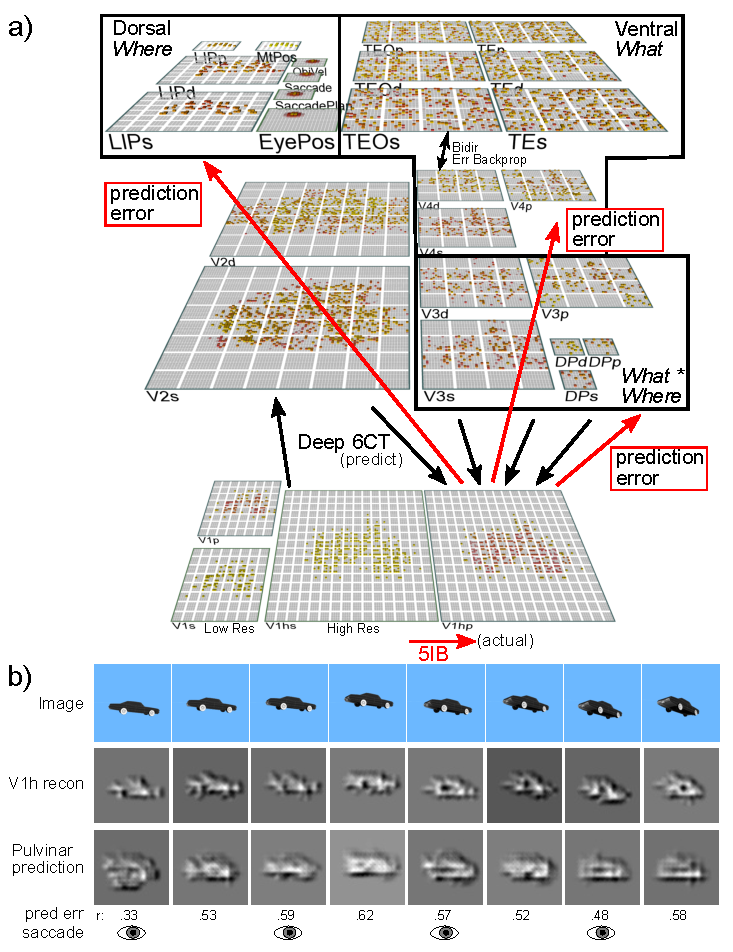
\includegraphics[width=4in]{figs/fig_deepleabra_wwi_ab_pred_model_frames}
  \caption{{\bf a)} The \emph{What-Where-Integration, WWI} model. The dorsal \emph{Where} pathway learns first, using easily-abstracted \emph{spatial blobs}, to predict object location based on prior motion, visual motion, and saccade efferent copy signals.  This drives strong top-down inputs to lower areas with accurate spatial predictions, leaving the \emph{residual} error concentrated on \emph{What} and \emph{What * Where} integration.  The V3 and DP (dorsal prelunate) constitute the \emph{What * Where} integration pathway, binding features and locations.  V4, TEO, and TE are the \emph{What} pathway, learning abstracted object category representations, which also drive strong top-down inputs to lower areas.  \emph{s} suffix = superficial, \emph{d} = deep, \emph{p} = pulvinar. {\bf c)} Example sequence of 8 alpha cycles that the model learned to predict, with the reconstruction of each image based on the V1 gabor filters (\emph{V1 recon}), and model-generated prediction (correlation $r$ prediction error shown).  The low resolution and reconstruction distortion impair visual assessment, but $r$ values are well above the $r$'s for each V1 state compared to the previous time step (mean = .38, min of .16 on frame 4 -- see SI for more analysis).  Eye icons indicate when a saccade occurred.}
  \label{fig.model}
\end{figure}

A critical question for predictive learning is whether it can develop high-level, abstract ways of representing the raw sensory inputs, while learning from nothing but predicting these low-level visual inputs.  For instance, can predictive learning really eliminate the need for human-labeled image datasets where abstract category information is explicitly used to train object recognition models via error-backpropagation?  Existing predictive-learning models based on error backpropagation \cite{LotterKreimanCox16} have not demonstrated the development of abstract, categorical representations.  Previous work has shown that predictive learning can be a useful method for pretraining networks that are subsequently trained using human-generated labels, but here we focus on the formation of systematic categories \emph{de-novo}.

To determine if our biologically based predictive learning model (Figure~\ref{fig.model}b) can naturally form such categorical encodings in the complete absence of external category labels, we showed the model brief movies of 156 3D object exemplars drawn from 20 different basic-level categories (e.g., car, stapler, table lamp, traffic cone, etc.) selected from the CU3D-100 dataset \cite{OReillyWyatteHerdEtAl13}.  The objects moved and rotated in 3D space over 8 movie frames, where each frame was sampled at the alpha frequency (Figure~\ref{fig.model}c).  There were also saccadic eye movements every other frame, introducing an additional predictive-learning challenge.  An efferent copy signal enabled full prediction of the effects of the eye movement, and allows the model to capture \emph{predictive remapping} (a widely-studied signature of predictive learning in the brain) \cite{DuhamelColbyGoldberg92,CavanaghHuntAfrazEtAl10}, and introduces additional predictive-learning challenge.  The only learning signal available to the model was a prediction error generated by the temporal difference between what it predicted to see in the next frame and what was actually seen.

\begin{figure}
  \centering\includegraphics[width=6in]{figs/fig_deepleabra_wwi_rsa_leabra_expt1}
  \caption{{\bf a)} Category similarity structure that developed in the highest layer, TE, of the biologically based predictive learning model, showing \emph{1-correlation} similarity of the TE representation for each 3D object against every other 3D object (156 total objects). Blue cells have high similarity, and model has learned block-diagonal clusters or categories of high-similarity groupings, contrasted against dissimilar off-diagonal other categories.  Clustering maximized average \emph{within - between} correlation distance (see SI).  All items from the same basic-level object categories (N=20) are reliably subsumed within learned categories. {\bf b)} Human similarity ratings for the same 3D objects, presented with the V1 reconstruction (see Fig 1c) to capture coarse perception in model, aggregated by 20 basic-level categories.  Each cell is 1 - proportion of time given object pair was rated more similar than another pair (see SI).  The human matrix shares the same centroid categorical structure as the model (confirmed by permutation testing and agglomorative cluster analysis, see SI).  {\bf c)} Emergence of abstract category structure over the hierarchy of layers.  Red line = correlation similarity between the TE similarity matrix (shown in panel a) and all layers; black line shows correlation similarity between V1 against all layers (1 = identical; 0 = orthogonal). Both show that IT layers (TEO, TE) progressively differentiate from raw input similarity structure present in V1, and, critically, that the model has learned structure beyond that present in the input.}
  \label{fig.rsa}
\end{figure}

We performed a representational similarity analysis (RSA) on the learned activity patterns at each layer in the model, and found that the highest IT layer (TE) produced a systematic organization of the 156 3D objects into 5 categories (Figure~\ref{fig.rsa}a), which visually correspond to the overall shape of the objects (pyramid-shaped, vertically-elongated, round, boxy / square, and horizontally-elongated). This organization of the objects matches that produced by humans making shape similarity judgments on the same set of objects, using the V1 reconstruction as shown in Figure~\ref{fig.model}c to capture the model's coarse-grained perception (Figure~\ref{fig.rsa}b; see supporting information for methods and further analysis).  Critically, Figure~\ref{fig.rsa}c shows that the overall similarity structure present in IT layers (TEO, TE) of the biological model is significantly different from the similarity structure at the level of the V1 primary visual input.  Thus the model, despite being trained only to generate accurate visual input-level predictions, has learned to represent these objects in an abstract way that goes beyond the raw input-level information.  Furthermore, this abstract category organization reflects the overall visual shapes of the objects as judged by human participants, suggesting that the model is extracting geometrical shape information that is invariant to the differences in motion, rotation, and scaling that are present in the V1 visual inputs.  We further verified that at the highest IT levels in the model, a consistent, spatially-invariant representation is present across different views of the same object (e.g., the average correlation across frames within an object was .901).  This is also evident in Figure~\ref{fig.rsa}a by virtue of the close similarity across multiple objects within the same category.

\begin{figure}
  \centering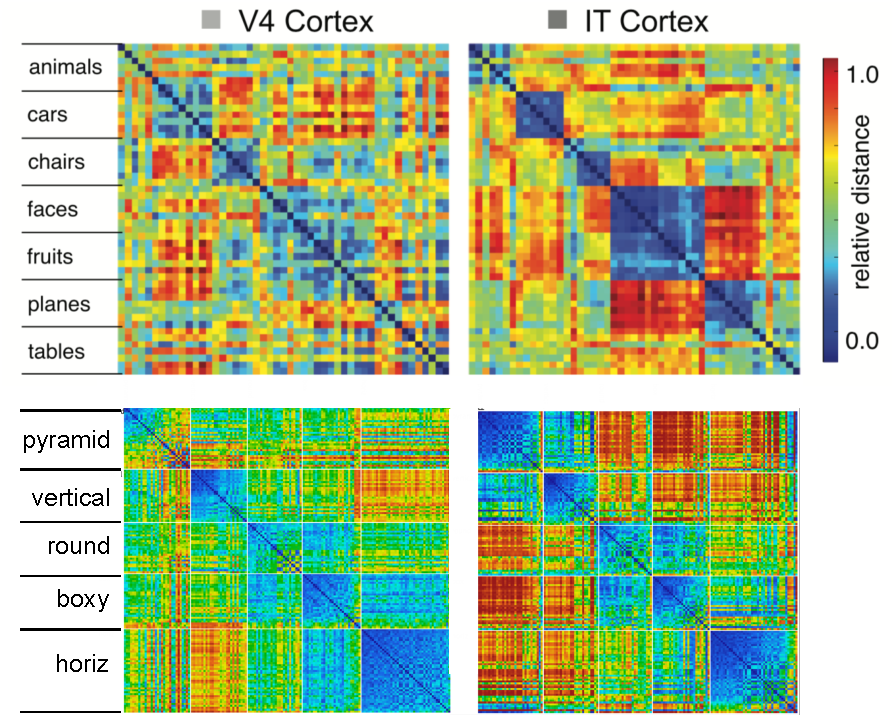
\includegraphics[width=4in]{figs/fig_deepleabra_wwi_rsa_leabra_macaque}
  \caption{Comparison of progression from V4 to IT in macaque monkey visual cortex (top row, from Cadieu et al., 2014) versus same progression in model (replotted using comparable color scale).  Although the underlying categories are different, and the monkeys have a much richer multi-modal experience of the world to reinforce categories such as foods and faces, the model nevertheless shows a similar qualitative progression of stronger categorical structure in IT, where the block-diagonal highly similar representations are more consistent across categories, and the off-diagonal differences are stronger and more consistent as well (i.e., categories are also more clearly differentiated).  Note that the critical difference in our model versus those compared in Cadieu et al. 2014 and related papers is that they explicitly trained their models on category labels, whereas our model is \emph{entirely self-organizing} and has no external categorical training signal.}
  \label{fig.macaque}
\end{figure}

Further evidence for the progressive nature of representation development in our model is shown in Figure~\ref{fig.macaque}, which compares the similarity structures in layers V4 and IT in macaque monkeys \cite{CadieuHongYaminsEtAl14} with those in corresponding layers in our model.  In both the monkeys and our model, the higher IT layer builds upon and clarifies the noisier structure that is emerging in the earlier V4 layer.  Considerable other work has also compared DCNN representations with these same data from monkeys \cite{CadieuHongYaminsEtAl14}, but it is essential to appreciate that those DCNN models were explicitly trained on the category labels, making it somewhat less than surprising that such categorical representations developed.  By contrast, we reiterate that our model has discovered its categorical representations entirely on its own, with no explicit categorical inputs or training of any kind.

\begin{figure}
  \centering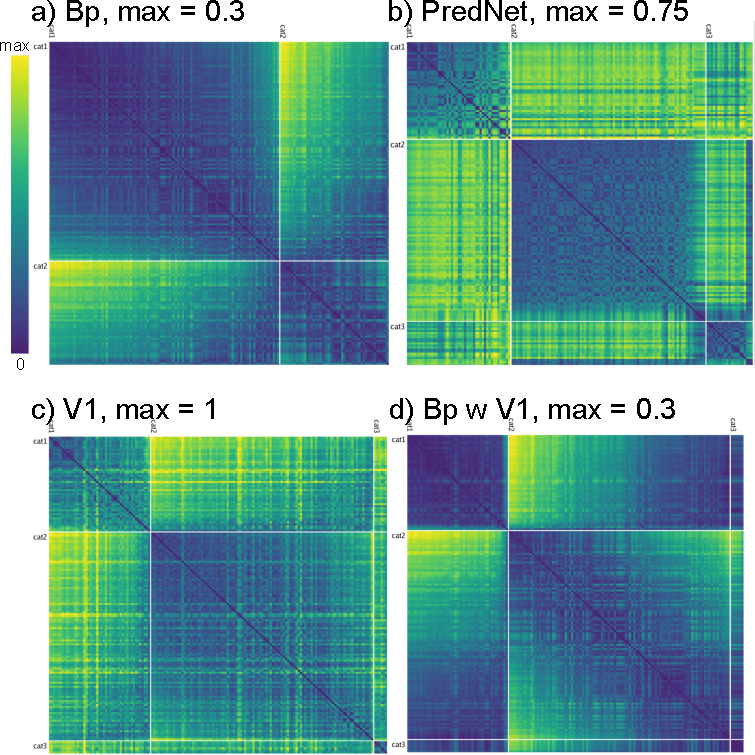
\includegraphics[width=4.5in]{figs/fig_deepleabra_wwi_bp_prednet_simat}
  \caption{{\bf a)} Best-fitting category similarity for TE layer of the backpropagation (Bp) model with the same What / Where structure as the biological model.  Only two broad categories are evident, and the lower \emph{max} distance (0.3 vs. 1.5 in biological model) means that the patterns are highly similar overall.  {\bf b)} Best-fitting similarity structure for the PredNet model, in the highest of its layers (layer 6), which is more differentiated than Bp (max = 0.75) but also less cleanly similar within categories (i.e., less solidly blue along the block diagonal), and overall follows a broad category structure similar to V1.  {\bf c)} Comparison of similarity structures across layers in the Bp model (compare to Figure~2c): unlike in the biological model, the V1 structure is largely preserved across layers, and is little different from the structure that best fits the TE layer shown in panel {\bf a}, indicating that the model has not developed abstractions beyond the structure present in the visual input.  Layer V3 is most directly influenced by spatial prediction errors, so it differs from both in strongly encoding position information.  {\bf d)} The best fitting V1 structure, which has 2 broad categories and banana is in a third category by itself.  The lack of dark blue on the block diagonal indicates that these categories are relatively weak, and every item is fairly dissimilar from every other.  {\bf e)} The same similarities shown in panel {\bf a} for Bp TE also fit reasonably well sorted according to the V1 structure (and they have a similar average within - between contrast differences, of 0.0838 and 0.0513 -- see SI for details).  {\bf f)} The similarity structure from the biological model resorted in the V1 structure does \emph{not} fit well: the blue is not aligned along the block diagonal, and the yellow is not strictly off-diagonal.  This is consistent with the large difference in average contrast distance: 0.5071 for the best categories vs. 0.3070 for the V1 categories.}
  \label{fig.bpred}
\end{figure}

Figure~\ref{fig.bpred} shows the results from a purely backpropagation-based (Bp) version of the same model architecture, and a standard PredNet model \cite{LotterKreimanCox16} with extensive hyperparameter optimization (see SI).  In the Bp model, the highest layers in the network form a simple binary category structure overall, and the detailed item-level similarity structure does not diverge significantly from that present at the lowest V1 inputs, indicating that it has not formed novel systematic structured representations, in contrast to those formed in the biologically based model.  Similar results were found in the PredNet model, where the highest layer representations remained very close to the V1 input structure.  Thus, it is clear that the additional biologically derived properties are playing a critical role in the development of abstract categorical representations that go beyond the raw visual inputs. These properties include: excitatory bidirectional connections, inhibitory competition, and an additional Hebbian form of learning that serves as a regularizer (similar to weight decay) on top of predictive error-driven learning \cite{OReilly98,OReillyMunakata00}.

Each of these properties could promote the formation of categorical representations. Bidirectional connections enable top-down signals to consistently shape lower-level representations, creating significant attractor dynamics that cause the entire network to settle into discrete categorical attractor states. By contrast, backpropagation networks typically lack these kinds of attractor dynamics, and this could contribute significantly to their relative lack of categorical learning.  Hebbian learning drives the formation of representations that encode the principal components of activity correlations over time, which can help more categorical representations coalesce (and results below already indicate its importance).  Inhibition, especially in combination with Hebbian learning, drives representations to specialize on more specific subsets of the space.  Ongoing work is attempting to determine which of these is essential in this case (perhaps all of them) by systematically introducing some of these properties into the backpropagation model, though this is difficult because full bidirectional recurrent activity propagation, which is essential for conveying error signals top-down in the biological network, is incompatible with the standard efficient form of error backpropagation, and requires much more computationally intensive and unstable forms of fully recurrent backpropagation \cite{WilliamsZipser92,Pineda87}.  Furthermore, Hebbian learning requires inhibitory competition which is difficult to incorporate within the backpropagation framework.

\begin{figure}
  \centering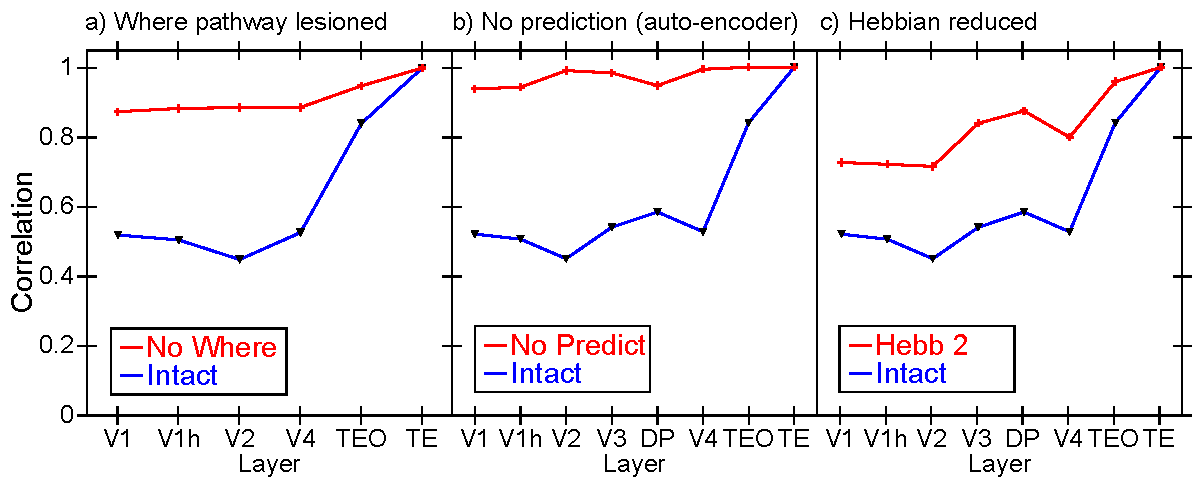
\includegraphics[width=4in]{figs/fig_deepleabra_wwi_leabra_manips}
  \caption{Effects of various manipulations on the extent to which TE representations differentiate from V1.  \emph{Std} is the same result shown in Figure 2c from the intact model for ease of comparison.  All of the following  manipulations significantly impair the development of abstract TE categorical representations (i.e., TE is more similar V1 and the other layers).  {\bf a)} Dorsal \emph{Where} pathway lesions, including lateral inferior parietal sulcus (LIP), V3, and dorsal prelunate (DP).  This pathway is essential for regressing out location-based prediction errors, so that the residual errors concentrate feature-encoding errors that train the \emph{What} pathway.  {\bf b)} Allowing the deep layers full access to current-time information, thus effectively eliminating the prediction demand and turning the network into an auto-encoder, which significantly impairs representation development, and supports the importance of the challenge of predictive learning for developing deeper, more abstract representations.  {\bf c)} Reducing the strength of Hebbian learning by 20\% (from 2.5 to 2), demonstrating the essential role played by this form of learning on shaping categorical representations.  Eliminating Hebbian learning entirely (not shown) prevented the model from learning anything at all, as it also plays a critical regularization and shaping role on learning.}
  \label{fig.manips}
\end{figure}

Figure~\ref{fig.manips} shows just a few of the large number of parameter manipulations that have been conducted to develop and test the final architecture.  For example, we hypothesized that separating the overall prediction problem between a spatial \emph{Where} vs. non-spatial \emph{What} pathway \cite{UngerleiderMishkin82,GoodaleMilner92}, would strongly benefit the formation of more abstract, categorical object representations in the \emph{What} pathway.  Specifically, the \emph{Where} pathway can learn relatively quickly to predict the overall spatial trajectory of the object (and anticipate the effects of saccades), and thus effectively regress out that component of the overall prediction error, leaving the residual error concentrated in object feature information, which can train the ventral \emph{What} pathway to develop abstract visual categories.  Figure~\ref{fig.manips}a shows that, indeed, when the \emph{Where} pathway is lesioned, the formation of abstract categorical representations in the intact \emph{What} pathway is significantly impaired.  Figure~\ref{fig.manips}b shows that full predictive learning, as compared to just encoding and decoding the current state (which is much easier computationally, and leads to much better overall accuracy), is also critical for the formation of abstract categorical representations --- prediction is a ``desirable difficulty'' \cite{Bjork94}.  Finally, Figure~\ref{fig.manips}c shows the impact of reducing Hebbian learning, which impairs category learning as expected.

\section{Predictive Saccade-driven Remapping}

A signature example of predictive behavior at the neural level in the brain is the {\em predictive remapping} of visual space in anticipation of a saccadic eye movements \cite{DuhamelColbyGoldberg92,ColbyDuhamelGoldberg97,GottliebKusunokiGoldberg98,NakamuraColby02,MarinoMazer16}.  Here, parietal neurons start to fire at the {\em future} receptive field location where a currently-visible stimulus will appear after a planned saccade is actually executed. Remapping has also been shown for border ownership neurons in V2 \cite{OHerronHeydt13} and in area V4 \cite{NeupaneGuittonPack16}. These are examples, we believe, of a predictive process operating throughout the neocortex to predict what will be experienced next.  A major consequence of this predictive process is the perception of a stable, coherent visual world despite constant saccades and other sources of visual change.  Our overall framework is consistent with the account of predictive remapping given by \incite{Wurtz08} and \incite{CavanaghHuntAfrazEtAl10}, who argue that the key remapping takes place at the high levels of the dorsal stream, which then drive top-down activation of the predicted location in lower areas, instead of the alternative where lower-levels remap themselves based on saccade-related signals.  The lower-level visual layers are simply too large and distributed to be able to remap across the relevant degrees of visual angle.


\section{Discussion}

In conclusion, we have demonstrated that learning based strictly on predicting what will be seen next is, in conjunction with a number of critical biologically motivated network properties and mechanisms, capable of generating abstract, invariant categorical representations of the overall shapes of objects.  The nature of these shape representations closely matches human shape similarity judgments on the same objects.  Thus, predictive learning has the potential to go beyond the surface structure of its inputs, and develop systematic, abstract encodings of the ``deeper'' structure of the environment.  Relative to existing machine-learning-based approaches in ``deep learning'', which have generally focused on raw categorization accuracy measures using explicit category labels or other human-labeled inputs, the results here suggest that focusing more on the nature of what is learned in the model might provide a valuable alternative approach.  Considerable evidence in cognitive neuroscience suggests that the primary function of the many nested (``deep'') layers of neural processing in the neocortex is to \emph{simplify} and aggressively \emph{discard} information \cite{SimonsRensink05}, to produce precisely the kinds of extremely valuable abstractions such as object categories, and, ultimately, symbol-like representations that support high-level cognitive processes such as reasoning and problem-solving \cite{RougierNoelleBraverEtAl05,OReillyPetrovCohenEtAl14}.  Thus, particularly in the domain of predictive or generative learning, the metric of interest should not be the accuracy of prediction itself (which is indeed notably worse in our biologically based model compared to the DCNN-based PredNet and backpropagation models), but rather whether this learning process results in the formation of simpler, abstract representations of the world that can in turn support higher levels of cognitive function.

% TODO
% * IssaCadieuDiCarlo18 -- predictive learning signals  -- need to see what this is actually

% * ERP N / P waves are exactly this.  also fixation timing etc.


In addition to the predictive learning functions of the deep / thalamic layers, these same circuits are also likely critical for supporting powerful top-down attentional mechanisms that have a net multiplicative effect on superficial-layer activations \cite{BortoneOlsenScanziani14,OlsenBortoneAdesnikEtAl12,BortoneOlsenScanziani14,OlsenBortoneAdesnikEtAl12}. The importance of the pulvinar for attentional processing has been widely documented \cite[e.g.,]{LaBergeBuchsbaum90,BenderYouakim01,SaalmannPinskWangEtAl12}, and there is likely an additional important role of the thalamic reticular nucleus (TRN), which can contribute a surround-inhibition contrast-enhancing effect on top of the incoming attentional signal from the cortex \cite{Crick84,Pinault04,WimmerSchmittDavidsonEtAl15}.  In our computational framework, these attentional modulation signals cause the iterative constraint satisfaction process in the superficial network to focus on task-relevant information while down-regulating responses to irrelevant information --- in the real world, there are typically too many objects to track at any given time, so predictive learning must be directed toward the most important objects. A subsequent paper will explore the attentional aspects of the DeepLeabra model and its synergy with the predictive learning aspect.


Considerable further work remains to be done to more precisely characterize the essential properties of our biologically motivated model necessary to produce this abstract form of learning, and to further explore the full scope of predictive learning across different domains.  We strongly suspect that extensive cross-modal predictive learning in real-world environments, including between sensory and motor systems, is a significant factor in infant development and could greatly multiply the opportunities for the formation of higher-order abstract representations that more compactly and systematically capture the structure of the world \cite{YuSmith12}.  Future versions of these models could thus potentially provide novel insights into the fundamental question of how deep an understanding a pre-verbal human, or a non-verbal primate, can develop \cite{SpelkeBreinlingerMacomberEtAl92,ElmanBatesKarmiloff-SmithEtAl96}, based on predictive learning mechanisms.  This would then represent the foundation upon which language and cultural learning builds, to shape the full extent of human intelligence.


\bibliography{ccnlab}

\end{document}
